
\begin{slide}
\heading{Tuning experiments}

%We start by considering how many tasks to include.  

The graph on the next slide considers the number of tasks to use.
%
\begin{itemize}
\item Each observation uses a fixed number of 64 workers;

\item Each plot uses a different value for $n$ (the number of intervals in the
  calculation), and repeats the integral $2^{28}/n$ times;

\item For each plot, we consider a variable number of tasks (expressed as the
average number of tasks per worker).
\end{itemize}
\end{slide}

%%%%%

\begin{slide}
% scala -cp .:/home/gavinl/Scala/SCL:/home/gavinl/Scala/Util
% TrapeziumExperiment  --doBagNumTasks --server --strict --buffering 16 on
% casteret 
\begin{tikzpicture}
\begin{semilogxaxis}[
%  title = Timing experiment on the numerical integration example,
  ylabel = Time (ms),
  legend pos = north east,
  height = 0.98\textheight,
  width = 0.98\textwidth,
  scaled ticks = false,
%  title = Experiment on the numerical integration bag-of-tasks example considering the number of tasks.,
  xlabel = Tasks per worker,
  log basis x=2,
  ymax = 4000
]
\input{TrapeziumExperiments/trapeziumBagExperimentBody}
\end{semilogxaxis}
\end{tikzpicture}
\end{slide}

%% \begin{slide}
%% % scala TrapeziumExperiment --doBagNumTasks --strict --server
%% % on aragorn
%% \begin{tikzpicture}
%% \begin{semilogxaxis}[
%%   ylabel = Time (ms),
%%   legend pos = north east,
%%   height = 0.98\textheight,
%%   width = 0.98\textwidth,
%%   scaled ticks = false,
%% %  title = Experiment on the numerical integration bag-of-tasks example considering the number of tasks.,
%%   xlabel = Tasks per worker,
%%   log basis x=2,
%%   ymax = 4000
%% ]
%% \addplot+[error bars/.cd, y dir=both,y explicit] coordinates {
%%   (1,2383.5665983333333) +- (0,23.80613532387126)
%%   (2,3488.652894125) +- (0,33.69172008103999)
%%   (4,5484.843809285714) +- (0,52.77587269901638)
%% };
%% \addlegendentry{$2^{18}$}
%% \addplot+[error bars/.cd, y dir=both,y explicit] coordinates {
%%   (1,1502.8543000816326) +- (0,14.886445138781143)
%%   (2,1385.2637562142856) +- (0,13.524033960637949)
%%   (4,1704.748456090909) +- (0,16.629363198523787)
%%   (8,2641.065219714286) +- (0,22.008531240160806)
%%   (16,4674.6223112) +- (0,44.736968547437314)
%% };
%% \addlegendentry{$2^{20}$}
%% \addplot+[error bars/.cd, y dir=both,y explicit] coordinates {
%%   (1,1301.1299476400002) +- (0,21.668929822917022)
%%   (2,1158.7164594600001) +- (0,20.63491724136467)
%%   (4,1060.57371676) +- (0,14.897112261051513)
%%   (8,951.5142809523809) +- (0,9.457915909333831)
%%   (16,1431.3107666875) +- (0,13.696011192633437)
%%   (32,2453.3797386) +- (0,22.591228481441735)
%%   (64,4401.394187181818) +- (0,40.48722292698239)
%% };
%% \addlegendentry{$2^{22}$}
%% \addplot+[error bars/.cd, y dir=both,y explicit] coordinates {
%%   (1,1246.97123994) +- (0,39.79525038997515)
%%   (2,1038.51840644) +- (0,22.29692535355058)
%%   (4,999.5409664199999) +- (0,15.21228289387058)
%%   (8,947.29102168) +- (0,16.46596672890571)
%%   (16,928.7719815199999) +- (0,11.096911610414564)
%%   (32,884.08558664) +- (0,13.321961813109784)
%%   (64,1364.3902661111113) +- (0,13.29697064254616)
%%   (128,2359.0651444) +- (0,23.50611978797186)
%%   (256,4314.4165685) +- (0,38.814383276837205)
%% };
%% \addlegendentry{$2^{24}$}
%% \addplot+[error bars/.cd, y dir=both,y explicit] coordinates {
%%   (1,1120.84683708) +- (0,27.79875556058014)
%%   (2,971.9654804600001) +- (0,19.691341803711843)
%%   (4,897.66914912) +- (0,17.205453545927018)
%%   (8,902.94097576) +- (0,18.19382426951521)
%%   (16,917.71139122) +- (0,14.540668378907382)
%%   (32,885.21201628) +- (0,17.333628626627796)
%%   (64,889.34188226) +- (0,15.904435087316362)
%%   (128,827.6861732333333) +- (0,7.775058441424386)
%%   (256,1327.3962545238094) +- (0,12.76074685830545)
%% };
%% \addlegendentry{$2^{26}$}
%% \addplot+[error bars/.cd, y dir=both,y explicit] coordinates {
%%   (1,1082.0089386341465) +- (0,10.819591155044764)
%%   (2,927.0113652599999) +- (0,12.370800929259476)
%%   (4,829.34869064) +- (0,14.556629683795158)
%%   (8,795.37391784) +- (0,14.74488349624712)
%%   (16,818.28530916) +- (0,22.33226507944289)
%%   (32,827.13741658) +- (0,17.009295410183945)
%%   (64,827.51467634) +- (0,17.64988040343166)
%%   (128,800.0242356599999) +- (0,19.928411650662497)
%%   (256,819.4069884600001) +- (0,13.921382946479966)
%% };
%% \addlegendentry{$2^{28}$}
%% \end{semilogxaxis}
%% \end{tikzpicture}
%% \end{slide}

%%%%%

\begin{slide}
\heading{Interpreting the results}

\begin{itemize}
\item Most of the plots have an initial downwards slope: having more tasks
gives more scope for load balancing.

\item Most of the plots hit a threshold, after which the time rises sharply:
at this threshold, the communication time becomes the dominant factor.
Each threshold corresponds to a task taking about 2ms.

Informal profiling shows that with $n = 2^{18}$, 64 workers and 4096 tasks (64
tasks per worker), that each worker spends less than 1\% of its time
calculating the integral: most of its time is spent waiting for a task or
waiting to send its result back to the controller. 
% scala -cp .:/home/gavinl/Scala/CSO:/home/gavinl/Scala/Util TrapeziumRun -p
% 64 --bagOfTasks --profile --reps 50 --size 262144 --numTasks 4096

Communication is expensive: avoid having too many communications. 

\end{itemize}
\end{slide}

%%%%%

\begin{slide}
\heading{Varying the number of workers}

The graphs on the next two slides consider the effect of varying the number of
workers.
%
\begin{itemize}
\item Each plot chooses a particular value for $n$, and a particular number
|nTasks| of tasks; the integral is repeated $2^{28}/n$ times; in most cases
|nTasks| is chosen to correspond to the minimum point on the corresponding
plot of the previous graph.

\item For each plot, we consider a variable number of workers.
\end{itemize}
\end{slide}


%%%%%

%% scala -cp .:/home/gavinl/Scala/SCL:/home/gavinl/Scala/Util TrapeziumExperiment  --doBagNumWorkers --server --strict --buffering 16
%% Done on casteret.
\begin{slide}
\begin{tikzpicture}
\begin{semilogxaxis}[
%  title = Timing experiment on the numerical integration example,
  ylabel = Time (ms),
  legend pos = north east,
  height = 0.98\textheight,
  width = 0.98\textwidth,
  scaled ticks = false,
%  title = Experiment on the numerical integration bag-of-tasks example.,
  xlabel = Number of workers,
  log basis x=2,
  ymax = 3000
]
\input{TrapeziumExperiments/trapeziumBagNumsWorkersExperimentBody}
%% \addplot+[error bars/.cd, y dir=both,y explicit] coordinates {
%%   (1,20980.71687533333) +- (0,179.91728825063942)
%%   (2,10825.120407647059) +- (0,107.67124527110484)
%%   (4,5662.8737155555555) +- (0,48.881017487644876)
%%   (8,2931.2210574) +- (0,21.2176082016105)
%%   (16,1579.0356856666667) +- (0,14.824123072478303)
%%   (32,968.6580589090909) +- (0,9.667665553104046)
%%   (64,802.6420259032258) +- (0,7.9255365976834)
%%   (128,881.1985728666667) +- (0,8.602261874969852)
%%   (256,910.06942584) +- (0,9.04644408134274)
%% };
%% \addlegendentry{$n = 2^{28}$; $2^{15}$ tasks}
%% \addplot+[error bars/.cd, y dir=both,y explicit] coordinates {
%%   (1,21509.421204692306) +- (0,210.65234399444674)
%%   (2,11100.843386642857) +- (0,106.58508810249897)
%%   (4,5979.9669022) +- (0,33.93849592352938)
%%   (8,3157.3363138) +- (0,23.074864083810652)
%%   (16,2029.1171042592591) +- (0,20.035747129164974)
%%   (32,2474.05068725) +- (0,24.28260348556887)
%%   (64,2323.5097085) +- (0,22.26944005506887)
%%   (128,2296.476720181818) +- (0,22.519422860666477)
%%   (256,2307.589541642857) +- (0,21.377616341076223)
%% };
%% \addlegendentry{$n = 2^{26}$; $2^{15}$ tasks}
%% \addplot+[error bars/.cd, y dir=both,y explicit] coordinates {
%%   (1,21301.226795333332) +- (0,199.62520021051938)
%%   (2,11008.6667308) +- (0,107.87620345833835)
%%   (4,5739.210235153846) +- (0,53.60834195284091)
%%   (8,2960.576561) +- (0,20.2911279533887)
%%   (16,1594.078433375) +- (0,14.909562315969149)
%%   (32,985.8041844666667) +- (0,9.647515407238965)
%%   (64,813.2873866315789) +- (0,7.949000996184872)
%%   (128,883.5242748974359) +- (0,8.794644861778885)
%%   (256,930.94703578) +- (0,9.248041427282121)
%% };
%% \addlegendentry{$n = 2^{26}$; $2^{13}$ tasks}
% \addplot+[error bars/.cd, y dir=both,y explicit] coordinates {
%   (1,19676.190000799998) +- (0,180.38188376457268)
%   (2,10425.489256545454) +- (0,98.73922761795579)
%   (4,5594.663830923077) +- (0,54.90413540417887)
%   (8,2950.0243936666666) +- (0,29.257502731295105)
%   (16,1593.7096355384615) +- (0,15.733255379405863)
%   (32,1024.6661964) +- (0,15.208727450799147)
%   (64,896.168408) +- (0,20.40659921715346)
%   (128,949.11078602) +- (0,19.65747010167658)
%   (256,1019.57806768) +- (0,22.475317644863118)
% };
% \addlegendentry{$n = 2^{26}$; $2^{11}$ tasks}
%% \addplot+[error bars/.cd, y dir=both,y explicit] coordinates {
%%   (1,21477.98017246154) +- (0,210.55285613699874)
%%   (2,11388.236008619047) +- (0,112.8923230663498)
%%   (4,5824.2682411999995) +- (0,54.05878986259698)
%%   (8,2996.027508125) +- (0,25.86268527087471)
%%   (16,1638.452026375) +- (0,15.395297671001751)
%%   (32,1040.65402518) +- (0,11.758960122039072)
%%   (64,879.0802259) +- (0,10.500830663423343)
%%   (128,951.91767112) +- (0,14.377880460923253)
%%   (256,1074.4891128800002) +- (0,12.570634159295883)
%% };
%% \addlegendentry{$n = 2^{24}$; $2^{11}$ tasks}
%% \addplot+[error bars/.cd, y dir=both,y explicit] coordinates {
%%   (1,21874.039732076923) +- (0,214.00187959121521)
%%   (2,11888.410480653847) +- (0,115.23120965428959)
%%   (4,5889.3582606) +- (0,58.47239060002575)
%%   (8,3058.0539968000003) +- (0,26.740352475594744)
%%   (16,1682.19076375) +- (0,15.88192182213644)
%%   (32,1102.5508139) +- (0,10.424344851002308)
%%   (64,952.0283832258065) +- (0,9.251155381500077)
%%   (128,1133.555203903226) +- (0,11.04517765126721)
%%   (256,1456.3417323333333) +- (0,14.401610336391443)
%% };
%% \addlegendentry{$n = 2^{22}$; $2^{9}$ tasks}
\end{semilogxaxis}
\end{tikzpicture}
\end{slide}

%%%%%%%%%%%%%%%%%%%%%%%%%%%%%%%%%%%%%%%%%%%%%%%%%%%%%%%%%%%%


\begin{slide}
\begin{tikzpicture}
\begin{axis}[
%  title = Timing experiment on the numerical integration example,
  ylabel = Time (ms),
  legend pos = north east,
  height = 0.98\textheight,
  width = 0.98\textwidth,
  scaled ticks = false,
%  title = Experiment on the numerical integration bag-of-tasks example.,
  xlabel = Number of workers
]
\addplot+[error bars/.cd, y dir=both,y explicit] coordinates {
  (32,1057.16423076) +- (0,9.058577712197186)
  (36,999.74580553) +- (0,11.645177559116714)
  (40,973.1374379800001) +- (0,11.456198170839446)
  (44,953.78469691) +- (0,12.728590553603095)
  (48,916.9048307200001) +- (0,11.70233118263378)
  (52,894.4999648200001) +- (0,12.11678851431492)
  (56,870.0977646900001) +- (0,11.748457689304136)
  (60,845.7953214099999) +- (0,11.289802513535895)
  (61,832.42320576) +- (0,11.7108890511239)
  (62,835.80386751) +- (0,12.138689555832116)
  (63,839.99481164) +- (0,11.672421013590865)
  (64,819.25139967) +- (0,10.387067101458893)
  (65,844.75961236) +- (0,12.801093903541023)
  (66,845.9632685700001) +- (0,12.471966782596876)
  (67,847.35187312) +- (0,10.672892815007007)
  (68,845.9432718200001) +- (0,11.687068136575018)
  (72,891.83480474) +- (0,11.664077754487357)
  (76,904.8890666699999) +- (0,13.849333784364212)
  (80,910.643654) +- (0,14.958665411558613)
  (84,925.2105237999999) +- (0,13.370598327925451)
  (88,933.76156279) +- (0,13.03384523365691)
  (92,945.99416009) +- (0,14.004558500497724)
  (96,935.03278638) +- (0,15.46433561441968)
};
\addlegendentry{$n = 2^{28}$; $2^{11}$ tasks}
\addplot+[error bars/.cd, y dir=both,y explicit] coordinates {
  (32,1047.0036780599999) +- (0,10.12864953178619)
  (36,1017.47902461) +- (0,8.928599779660411)
  (40,959.36274902) +- (0,11.548453150543029)
  (44,939.42318046) +- (0,10.66254931143366)
  (48,920.41573693) +- (0,10.981041832845595)
  (52,875.13599263) +- (0,10.995263114175062)
  (56,857.05920759) +- (0,11.880093324880574)
  (60,838.76808737) +- (0,11.966432737920348)
  (61,837.19906271) +- (0,10.994746674812482)
  (62,822.75986079) +- (0,11.560733547555344)
  (63,838.5286888400001) +- (0,12.547840528475888)
  (64,822.0841385900001) +- (0,10.754504325423445)
  (65,839.47520976) +- (0,10.85184114086948)
  (66,837.2459781) +- (0,10.74095667831926)
  (67,841.43561061) +- (0,11.832395940633196)
  (68,836.63884214) +- (0,10.928017252652067)
  (72,862.02357001) +- (0,10.918237896447021)
  (76,884.6797420700001) +- (0,13.341316678584352)
  (80,893.05673185) +- (0,12.620337768215595)
  (84,905.3931114) +- (0,14.815073165280992)
  (88,912.07447821) +- (0,15.037886194336814)
  (92,923.2464966599999) +- (0,14.14010852955829)
  (96,932.22233657) +- (0,16.126199487105648)
};
\addlegendentry{$n = 2^{28}$; $2^{12}$ tasks}
\addplot+[error bars/.cd, y dir=both,y explicit] coordinates {
  (32,970.01944693) +- (0,7.921036621992584)
  (36,914.78684992) +- (0,6.249635136929345)
  (40,878.2211187) +- (0,6.002492317074767)
  (44,854.85132241) +- (0,5.805545823912017)
  (48,830.9678371699999) +- (0,5.679552383901102)
  (52,817.20496864) +- (0,9.03952819717361)
  (56,807.67801987) +- (0,10.671596046890532)
  (60,794.73721048) +- (0,11.403890485450642)
  (61,792.36021697) +- (0,9.63988417250338)
  (62,799.04136866) +- (0,9.316949146902312)
  (63,811.32646775) +- (0,11.511590899864105)
  (64,799.99827983) +- (0,11.348725846788136)
  (65,827.3647095900001) +- (0,11.570706095405262)
  (66,838.74349195) +- (0,10.179701089001567)
  (67,848.0990576900001) +- (0,10.810667215305367)
  (68,848.1674477400001) +- (0,10.072236809703199)
  (72,866.80552821) +- (0,12.81106123636495)
  (76,873.29217525) +- (0,11.142424555824947)
  (80,891.38543958) +- (0,12.391723956860375)
  (84,912.0764636900001) +- (0,12.390811540406208)
  (88,914.1266091499999) +- (0,10.452233049440322)
  (92,916.00132452) +- (0,12.395476534616462)
  (96,916.9366761699999) +- (0,11.524883867646627)
};
\addlegendentry{$n = 2^{28}$; $2^{13}$ tasks}
\addplot+[error bars/.cd, y dir=both,y explicit] coordinates {
  (32,967.38429043) +- (0,5.228718418500252)
  (36,917.75526807) +- (0,4.902219191042896)
  (40,876.2538620800001) +- (0,4.894228134218586)
  (44,856.3277520199999) +- (0,5.958682903059108)
  (48,829.02229928) +- (0,5.5045836608205025)
  (52,811.75331553) +- (0,7.835844147933334)
  (56,786.6318125) +- (0,8.641143824325146)
  (60,779.9289284299999) +- (0,8.678707450542706)
  (61,777.5527782) +- (0,9.79110552822866)
  (62,787.7280826900001) +- (0,10.12832921663263)
  (63,816.3992593500001) +- (0,10.117377174458076)
  (64,805.95226873) +- (0,11.017142834750626)
  (65,876.17967412) +- (0,8.704983651904703)
  (66,904.26515138) +- (0,6.45277015673139)
  (67,905.14452448) +- (0,7.124153235033365)
  (68,912.69245073) +- (0,7.176631192178639)
  (72,920.8256426900001) +- (0,6.612147300010088)
  (76,923.86468353) +- (0,7.392114375370194)
  (80,921.9161873099999) +- (0,7.573687495256987)
  (84,932.63994972) +- (0,6.631146953020805)
  (88,925.26523717) +- (0,7.212872863077761)
  (92,930.39899885) +- (0,7.510944935957713)
  (96,931.4948726499999) +- (0,6.721705426187553)
};
\addlegendentry{$n = 2^{28}$; $2^{14}$ tasks}
\addplot+[error bars/.cd, y dir=both,y explicit] coordinates {
  (32,974.32503694) +- (0,5.744042307420299)
  (36,925.96370338) +- (0,5.836374502816456)
  (40,881.75518242) +- (0,5.082751337706672)
  (44,850.57672641) +- (0,5.132371111165055)
  (48,821.53729789) +- (0,5.057809120336692)
  (52,794.06088546) +- (0,4.563300268250611)
  (56,792.39804285) +- (0,5.530226710785223)
  (60,799.4750715567011) +- (0,3.9938417684203933)
  (61,802.61271401) +- (0,4.662692237628614)
  (62,800.4614891599999) +- (0,4.296707552469622)
  (63,802.2559684700001) +- (0,4.179250629400057)
  (64,801.04295838) +- (0,4.061202020040299)
  (65,808.2957718600001) +- (0,4.837913031278439)
  (66,808.72313119) +- (0,4.199804487372714)
  (67,815.0734691900001) +- (0,4.137220500208479)
  (68,818.91990154) +- (0,4.563271772796916)
  (72,824.6117649081633) +- (0,4.087151944038204)
  (76,833.09898537) +- (0,5.1750502874207)
  (80,835.74869213) +- (0,4.819153404466759)
  (84,841.59737972) +- (0,5.131775161182797)
  (88,851.22751764) +- (0,5.582829491779009)
  (92,851.79473028) +- (0,5.489386416048899)
  (96,854.1576239) +- (0,5.723156516817434)
};
\addlegendentry{$n = 2^{28}$; $2^{15}$ tasks}
\end{axis}
\end{tikzpicture}
\end{slide}

%%%%%

\begin{slide}
\heading{Interpreting the results}

Most of the plots have a minimum with about 62 workers (plus the distributor
and collector), matching the number of machine threads.  (In the second graph,
the confidence intervals overlap, so we can't be sure about the precise
position of the minimum.)

%% One exception is where there are insufficient tasks per worker to
%% achieve good load balancing, so there's a bit of a fall-off in
%% performance.

%% Another exception is a case where there are too many tasks, and so the
%% communication overheads dominate.
%% Communication is expensive: avoid having too many communications. 

Note that the running times are 15--20\% faster than on
slide~\ref{slide:not-bag-of-tasks}: the bag-of-tasks technique works!
\end{slide}
